\documentclass{beamer}

%\usepackage{minted}
\usepackage{xltxtra}
\usepackage{xgreek}
\usepackage{url}

%\usetheme{Copenhagen}
%\usetheme[roses]{boxes}
%\usetheme{Frankfurt}
%\usecolortheme{dolphin}
\usetheme{Warsaw}


%\setsansfont[Mapping=tex-text]{CMU Serif}
\setsansfont[Mapping=tex-text]{DejaVu Sans}

\author[afein,fedjo,mastergreg,mariaral]{Alex Maurogiannis, George Marinellis, Gregory Lyras, Maria Ralli}
\institute{CSlab @ NTUA}
\title{Cilk vs LU (tiled version)}
\subtitle{Part III}

\date{\today}


\begin{document}
\AtBeginSection[]
{
    \begin{frame}{Επισκόπηση}
        \tableofcontents[currentsection]
    \end{frame}
}
%--- the titlepage frame -------------------------%
\begin{frame}
    \titlepage
\end{frame}

\section{Περιγραφή Προσέγγισης}
\subsection{Tiles and Tasks}
\begin{frame}{tiles and tasks}
    \begin{quote}
        Στην tiled έκδοση σπάμε σε τμήματα τον αρχικό πίνακα μεγέθους block size
        και σε αυτά εκτελούμε περισσότερες αλλά απλούστερες πράξεις.
    \end{quote}
    \pause

    \begin{block}{Πράξεις ανά tile}
        \begin{enumerate}
            \item<2-> LU kernel on the diagonal tile
            \item<3-> Tile matrix inversion
            \item<4-> matrix multiplication of row and column
            \item<5-> matrix multiplication and update of the remaining tiles
            \item<6-> LU kernel on the final tile
            
        \end{enumerate}
    \end{block}

\end{frame}

\begin{frame}{tiles and tasks}
    \begin{block}{Παράδειγμα Εκτέλεσης}
        \includegraphics[width=\textwidth]{files/pps-ex2-pres_tables.png}
    \end{block}
\end{frame}

\begin{frame}{Γράφος εξαρτήσεων}
    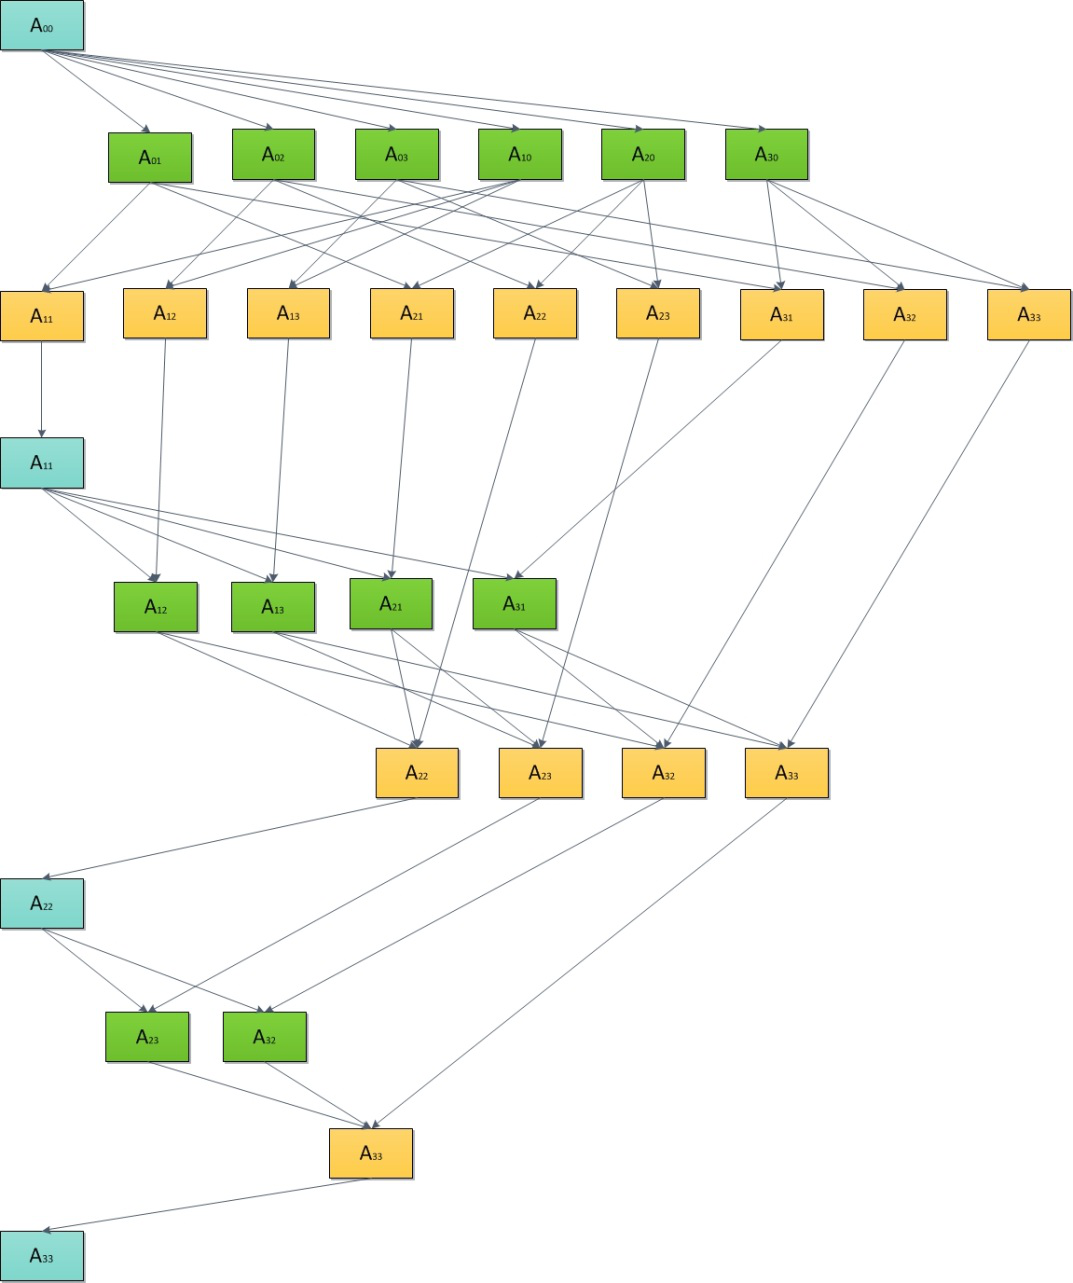
\includegraphics[height=\textheight]{files/task_graph_full.png}
\end{frame}
\subsection{Τελικές Εκδόσεις}
\begin{frame}{Τελικές Εκδόσεις}
    \begin{block}{Εκδόσεις }
        \begin{itemize}
                
            \item<1-> \begin{minipage}{0.7\textwidth}
                    Tiled με αναδρομικό for
                \end{minipage}
                \begin{minipage}[h]{0.1\textwidth}
                \begin{flushright}
                        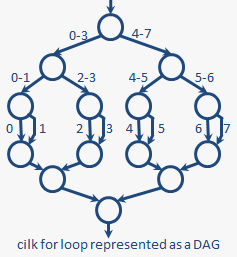
\includegraphics[scale=0.45]{files/rec_for.png}
                \end{flushright}
                \end{minipage}
                    \begin{itemize}
                        \item<2-> MIT cilk
                        \item<3-> gcc-cilkplus
                    \end{itemize}
            \item<4-> Tiled με χρήση cilk\_for
                \begin{itemize}
                    \item<5-> gcc-cilkplus
                \end{itemize}
            \item<6-> Task Graph
                \begin{itemize}
                    \item<7-> gcc-cilkplus
                \end{itemize}
        \end{itemize}
    \end{block}
\end{frame}



\section{Παρουσίαση Αποτελεσμάτων}

\subsection{Επιλογή Block Size}
    \begin{frame}
        \begin{block}{Sandman Block Size Sweep}
            \begin{figure}[H]
                \centering
                \includegraphics[scale=0.23]{files/sandman_block_size_sweep_4k.png}
                \caption{4096 Matrix Size, 64 threads}
            \end{figure}
        \end{block}
    \end{frame}

    \begin{frame}
        \begin{block}{Clones Block Size Sweep}
            \begin{figure}[H]
                \centering
                \includegraphics[scale=0.23]{files/clones_block_size_sweep_4k.png}
                \caption{4096 Matrix Size, 8 threads}
            \end{figure}
        \end{block}
    \end{frame}

\subsection{Σύγκριση χρόνων και speedups}

\begin{frame}
    \begin{block}{LU tiled έκδοση με cilk\_for}
        \begin{figure}[H]
            \centering
            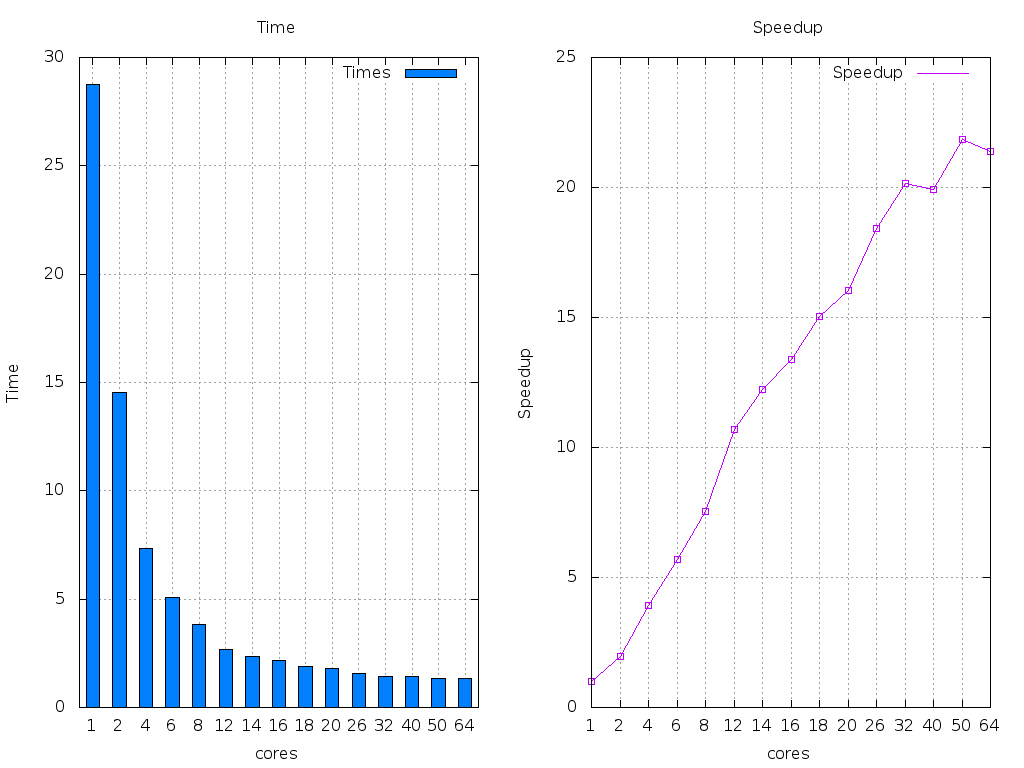
\includegraphics[scale=0.23]{files/sandman_tiled_cilk_for.png}
            \caption{4096 Matrix Size, 32 block size}
        \end{figure}
    \end{block}
\end{frame}

\begin{frame}
    \begin{block}{LU tiled με αναδρομικό for}
        \begin{figure}[H]
            \centering
            \includegraphics[scale=0.23]{files/sandman_tiled_cilkplus_rec_for.png}
            \caption{4096 Matrix Size, 32 block size}
        \end{figure}
    \end{block}
\end{frame}

\begin{frame}
    \begin{block}{αναδρομική tiled σε cilkplus vs cilk\_for}
        \begin{figure}[H]
            \centering
            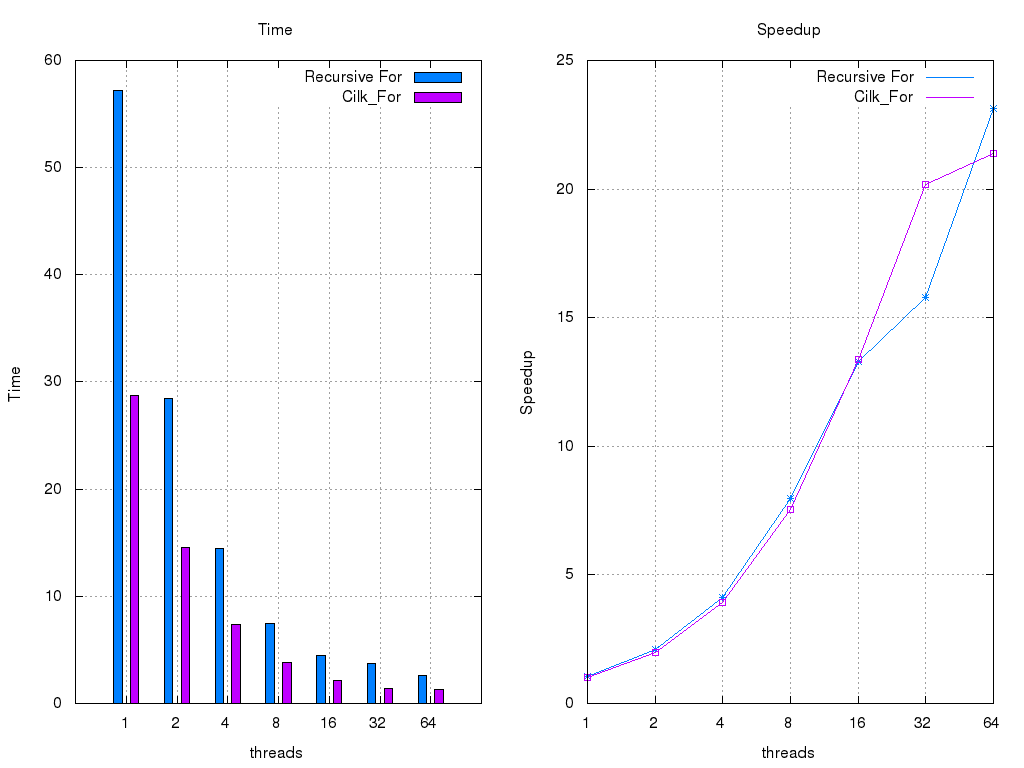
\includegraphics[scale=0.23]{files/sandman_tiled_for_comparison.png}
            \caption{4096 Matrix Size, 32 block size}
        \end{figure}
    \end{block}
\end{frame}

\begin{frame}
    \begin{block}{Task Graph}
        \begin{figure}[H]
            \centering
            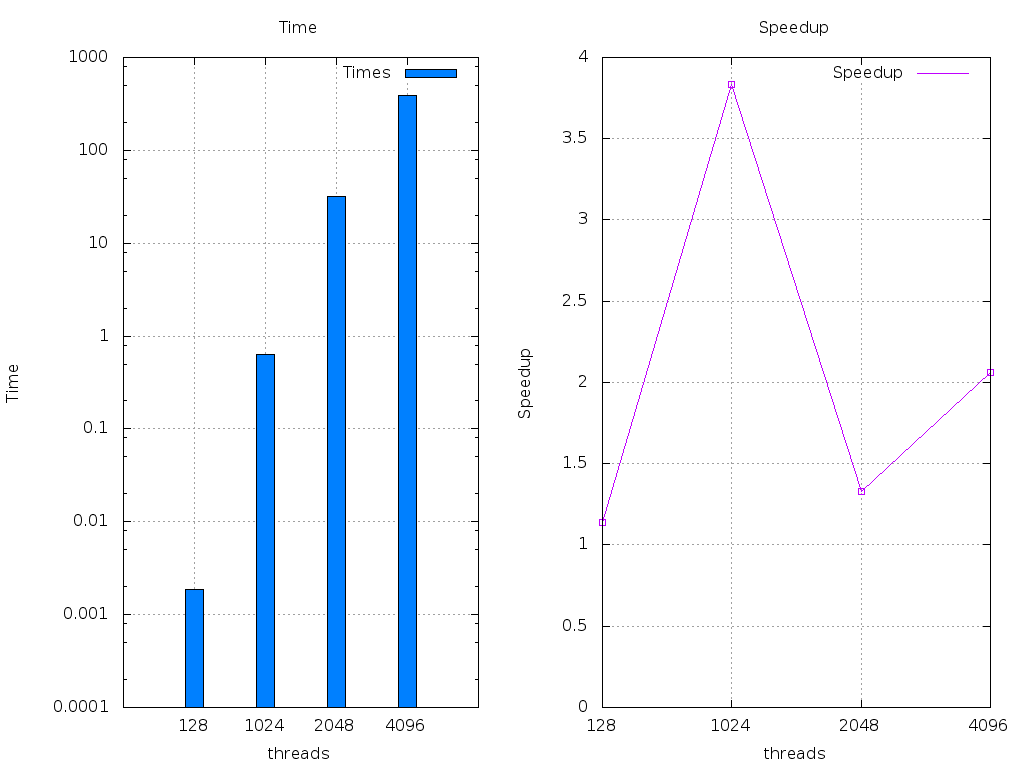
\includegraphics[scale=0.23]{files/clones_graph_tiled_times.png}
            \caption{8 threads, $block size = Matrix size /4$}
        \end{figure}
    \end{block}
\end{frame}

\section{Σύνοψη}

\subsection{Pitfalls to avoid}
\begin{frame}{Pitfalls}
    \begin{itemize}
            \item<1-> Στην Tiled έκδοση της LU παρατηρήσαμε μεγάλες τιμές
                σφαλμάτων που οφείλονται στο διαφορετικό τρόπο υπολογισμών
                πάνω σε αριθμούς κινητής υποδιαστολής.
            \item<2-> Το μέγεθος του block size έχει πολύ σημαντική επίδραση
                στις τιμές των παραπάνω σφαλμάτων και οποιαδήποτε
                βελτιστοποίηση καλό είναι να ελέγχεται ως προς την ακρίβειά
                της.
            \item<3-> Το μεγαλύτερο ποσοστό (άνω του 90\%) του χρόνου
                εκτέλεσης της tiled έκδοσης καταναλώνεται στον πολλαπλασιασμό
                και την ενημέρωση των tiles (βήμα 4) συνεπώς η παραλληλοποίηση
                πρέπει να είναι στοχευμένη σε αυτό το βήμα.
    \end{itemize}
\end{frame}


\subsection{Συμπεράσματα}
\begin{frame}{Συμπεράσματα}
    \begin{itemize}
            \item<1-> Το Block Size επιρρεάζει σημαντικά την επίδοση, πιο
                συγκεκριμένα, έχουμε βέλτιστη εκτέλεση με BS 32 ενώ πάνω από
                64 οι χρόνοι είναι απαγορευτικοί.
            \item<2-> Το cilk\_for παρουσιάζει μέγιστο speedup σε σύγκριση με
                τις υπόλοιπες tiled υλοποιήσεις.
            \item<3-> Η χρήση rec\_for δίνει αντίστοιχο speedup με διπλάσιο
                κόστος σε χρόνο.
            \item<4-> Το Task Graph επιτρέπει τη μέγιστη δυνατή παραλληλία του
                αλγορίθμου, ωστόσο ο στατικός γράφος εξαρτήσεων που
                χρησιμοποιήσαμε χαρακτηρίζεται από μικρό fan out και κατά
                συνέπεια από κακές επιδόσεις.
    \end{itemize}
\end{frame}

\begin{frame}{Τελική σύγκριση}
    Εδώ μπαίνει το διάγραμμα με όλες τις εκδόσεις
\end{frame}

\begin{frame}
    \begin{block}{Best of}
    \begin{itemize}
        \item<1-> Speedup:
            \begin{enumerate}
                \item<2-> First
                \item<3-> Second
                \item<4-> Third
            \end{enumerate}
        \item<5-> Time:
            \begin{enumerate}
                \item<6-> First
                \item<7-> Second
                \item<8-> Third
            \end{enumerate}
    \end{itemize}
    \end{block}
\end{frame}


\subsection{Ερωτήσεις}
\begin{frame}{Ερωτήσεις;;}
    Ask! :)
\end{frame}

\begin{frame}{Thanks}
    \begin{itemize}
        \item Thanks for watching
    \end{itemize}
\end{frame}

\end{document}
